\documentclass[UTF8]{ctexbook}
\usepackage{polyglossia}
\usepackage{tipa}
\usepackage{multicol}

\setotherlanguages{arabic}
\setotherlanguages{english}

\newfontfamily\arabicfont[Script=Arabic]{MicrosoftSansSerif}
\newfontfamily\arabicfontit[Script=Arabic]{WaseemLight}
% \newfontfamily\arabicfontit[Script=Arabic]{DiwanThuluth}
\newfontfamily\arabicfontbf[Script=Arabic]{DiwanKufi}

\newbool{innote}
\setbool{innote}{false}

\newenvironment{note}{
        \booltrue{innote}  
        \itshape
    }{
        \boolfalse{innote} 
    }


\newcommand{\arm}[1]{%
    \ifbool{innote}
        {\textarabic{\arabicfontit{#1}}}  % 在 note 环境中使用斜体
        {\textarabic{#1}}                 % 其他环境使用正常字体
}
% \newcommand{\arm}[1]{\textarabic{#1}}
\newcommand{\ait}[1]{\arabicfontit{#1}}
\newcommand{\abf}[1]{\arabicfontbf{#1}}
\newcommand{\ac}[2]{#2 \hspace{\stretch{1}} \arm{\Large #1}}

\title{\arm{\Huge \arabicfontbf{اَللُّغَةُ الْعَرَبِيَّةُ}} \\ 阿拉伯语笔记}
\author{}
\date{\today}
\begin{document}
\maketitle

\chapter*{前言}

\vfill
\begin{center}

    \arm{\ait {\Large اُطْلُبُوْا العِلْمَ وَلَوْ في الصِّينِ.}}
    
    ~\\

    \emph{求知,哪怕在中国。}
\end{center}
\vfill

\begin{center}
    \begin{center}
        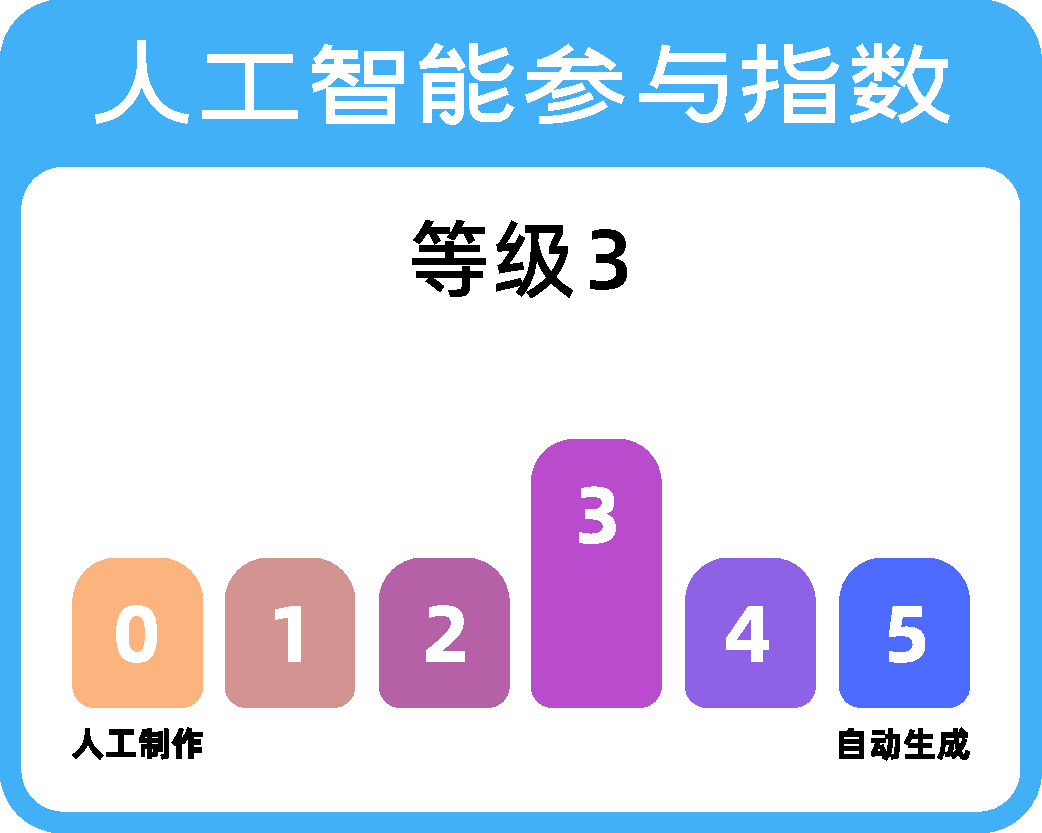
\includegraphics[width=0.4\textwidth]{img/iiia.pdf}
    \end{center}
\end{center}

本笔记借助了GitHub Copilot生成。这玩意太好用了,甚至能猜想到例句(不过发音符号有时会标错),我审核了AI生成的所有内容,但由于毕竟是新接触一套书写系统,难免有拼写疏漏。

\begin{attention}
    这样的格式代表老师在课上强调的知识点。
\end{attention}

\begin{note}
    这样的格式代表我自己的感悟。
\end{note}

\chapter{引言和字母表部分}

本章对应课程P1~P7。

\section{字母表(\arm{اَلْأَبْجَدِيَّةُ الْعَرَبِيَّةُ})及特殊字母写法}

\begin{note}
    字母表请务必跟着视频课学习。笔记只能呈现字母的部分形态。

    此外,在学习阿语字母表时,我愈发意识到,对于老师来说,阿语的一些字形可能已经很熟悉,因此讲解时会快速带过,或干脆略过。但我们来说,面对这样一款陌生的语言,我们需要尝试用最快的速度掌握分辨字形的合适粒度。也就是说,我们需要知道对于这套文字,哪些地方是装饰、哪些地方是区别字母的关键、哪些地方是字体的差异。

    举个例子,\arm{ل} 与 \arm{ا} 搭配而成的 \arm{لا} 有一个独特的词尾型 \arm{ـلا}。在字形呈现上, \arm{لا} 和 \arm{ـلا} 可能很相似,也可能相差很大。这是视频课中没有明确提到的,需要我们自己去观察发现。
\end{note}

\begin{Arabic}
    \begin{tabular}{c|r|r|r|r}
        \crm{独立型} & \crm{读音} & \crm{词头、中、尾连写} & \crm{誊抄} & \crm{特殊形态} \\
        \hline
        أ & أَلِفٌ & أـأـأ & \ait{أـأـأ} & إِ آ \\
        ب & بَاءٌ & بـبـب & \ait{ببب}\\
        ت & تَاءٌ & تـتـت & \ait{تتت} & ة/ـة ةََ \\
        ث & ثَاءٌ & ثـثـث & \ait{ثثث}\\
        ج & جِيمٌ & جـجـج & \ait{ججج}\\
        ح & حَاءٌ & حـحـح & \ait{ححح}\\
        خ & خَاءٌ (厚) & خـخـخ & \ait{خخخ}\\
        د & دَالٌ & دـدـد & \ait{دـدـد}\\
        ذ & ذَالٌ (咬) & ذـذـذ & \ait{ذـذـذ}\\
        ر & رَاءٌ (厚) & رـرـر & \ait{رـرـر}\\
        ز & زَاىٌ & زـزـز & \ait{زـزـز}\\
        س & سِينٌ & سـسـس & \ait{سسس}\\
        ش & شِينٌ & شـشـش & \ait{ششش}\\
        ص & صَادٌ (厚) & صـصـص & \ait{صصص}\\
        ض & ضَادٌ (厚) & ضـضـض & \ait{ضضض}\\
        ط & طَاءٌ (厚) & طـطـط & \ait{تتت}\\
        ظ & ظَاءٌ (厚/咬) & ظـظـظ & \ait{ظـظـظ}\\
        ع & عَينٌ & عـعـع & \ait{ععع}\\
        غ & غَينٌ & غـغـغ & \ait{غغغ}\\
        ف & فَاءٌ & فـفـف & \ait{ففف}\\
        ق & قَافٌ (厚) & قـقـق & \ait{ققق}\\
        ك & كَافٌ & كـكـك & \ait{ككك}\\
        ل & لَامٌ & لـلـل & \ait{للل} & لا/ـلا لاَ لاََ \\
        م & مِيمٌ & مـمـم & \ait{ممم}\\
        ن & نُونٌ & نـنـن & \ait{ننن}\\
        ه & هَاءٌ & هـهـه & \ait{ههه}\\
        و & وَاوٌ & وـوـو & \ait{وـوـو}\\
        ى & يَاءٌ & يـيـى & \ait{ييى}\\
    \end{tabular}
\end{Arabic}

\begin{itemize}
    \item 标``厚''表示其后加 \arm{ـَ} 或 \arm{ـَا} 时发音要更浑厚(靠后,类似\textipa{[A]})。
    \item 标``咬''表示咬舌发音。
    \item \arm{ة} 常位于词尾,一般为阴性名词标志,其前字母永远标 \arm{ـَ} 或 \arm{ـَا} 。\arm{ة} 搭配 \arm{ــََا} 时不写 \arm{ا}。
\end{itemize}

\begin{note}
    在学习满语时我发现,如果过多按照独立型去背诵字母形态,在识读单词的时候会遇到更大的障碍,因为单词中的单词大多数处于词中型。既然如此,为什么不按照词中型将字母整理出来呢?于是,便有了这个列表。

    我根据自己的理解,依照课上的手写体,给每个形状取了名字。此外,请注意阅读顺序(从两边到中间)。
    \begin{itemize}
        \item \ac{ـهـ و ـمـ}{(不规则)h, w, m}
        \item \ac{ـئـ / ـنـ ـتـ ـثـ / ـبـ ـيـ}{(短牙型)' / n, t, th / b, y}
        \item \ac{ـلـ ـكـ}{(长牙型)l, k}
        \item \ac{ـــحـ / ـــخـ / ـــجـ}{(闪电型)ḥ / kh / \textipa{\textdyoghlig}}
        \item \ac{د ذ / ر ز}{(小钩型)d, dh / r, z}
        \item \ac{ـسـ ـشـ}{(横线型)s, sh}
        \item \ac{ـفـ ـقـ / ـطـ ـظـ / ـصـ ـضـ}{(上圈型)f, q / ṭ, ẓ / ṣ, ḍ}
        \item \ac{ـعـ ـغـ}{(三角型)`, gh}
    \end{itemize}

    可以看到,转写中为拉丁字母加点,对应到阿文很可能会完全变成另一个字母。于是,我又整理了如下表格,来表示部分字母的发音关系。该表中,关于中心轴对称的辅音互为清浊关系。越远离中心轴,表示发音越难(加喉音、加顶音等)。对应转写并列展示。

    \begin{center}
    \begin{multicols}{2}
    \begin{tabular}{cc||cc}
        \hline
        \arm{ض} & \arm{د} & \arm{ت} & \arm{ط} \\
        && \arm{ك} & \arm{ق} \\
        & \arm{غ} & \arm{خ} \\
        \arm{ع} && \arm{ه} & \arm{ح}\\
        & \arm{ج} & \arm{ش} \\
        & \arm{ز} & \arm{س} & \arm{ص} \\
        \arm{ظ} & \arm{ذ} & \arm{ث} \\
        \hline
    \end{tabular}

    \begin{tabular}{cc||cc}
    
        \hline
        ḍ & d & t & ṭ \\
        && k & q \\
        & gh & kh \\
        ` && h & ḥ \\
        & \textipa{\textdyoghlig} & sh \\
        & z & s & ṣ \\
        ẓ & dh & th \\
        \hline

    \end{tabular}
    \end{multicols}
    \end{center}
\end{note}

\section{单词和课文}

\subsection{引入和字母部分}

\begin{itemize}
    \item \ac{اَلْعَرَبِيَّةُ}{阿拉伯语}
    \item \ac{اَلْبُلْدَانُ الْعَرَبِيَّةُ}{阿拉伯国家}
    \item \ac{صَحْرَاءُ}{沙漠}
    \item \ac{اَصَّحْرَاءُ الْكُبْرَى}{撒哈拉沙漠(沙漠--最大的)}
    \item \ac{جَمَلٌ}{骆驼}
    \item \ac{نِفْطٌ}{石油}
    \item \ac{بِتْرُولٌ}{石油(音译自petrol)}
    \item \ac{قَهْوَةٌ}{咖啡}
    \item \ac{أَلْفُ لَيْلَةِِ وَلَيْلَةٌ}{《一千零一夜》(一千--夜(属)--和一夜)}
    \item \ac{جُبْرَانُ}{纪伯伦}
    \item \ac{اَللُّغَاتُ السَّامِيَّةُ}{闪米特语族(Semitic Languages)}

\end{itemize}

\section{语法}

阿拉伯语属于闪含语系闪语族(闪米特语族),诞生于阿拉伯半岛,最早的文献可以追溯到公元6世纪阿拉伯半岛北部的石刻。

阿拉伯语辅音相对复杂,一般三个辅音字母构成基本含义。例如:

\begin{itemize}
    \item \ac{فَهِمَ}{理解}
    \item \ac{أَفِهَمَ}{使……理解}
    \item \ac{تَفَاهَمَ}{相互理解}
    \item \ac{اِسْتَفْهَمَ}{询问(要求理解)}
    \item \ac{مَفْهُومٌ}{概念(被理解的事物)}
\end{itemize}

阿拉伯语有名词、动词、虚词,没有系动词:

\begin{itemize}
    \item \ac{هَذَا كِتَابٌ.}{这--一本书。(\arm{هَذَا}注音为\arm{هَاذَا})}
\end{itemize}

阿语动词常在句首:遇到--张三(主格)--李四(宾格)

\chapter{hello, world}

\lecon{8.1}

\section{单词和课文}

\begin{itemize}
    \item \ac{أَهْلٌ}{家人}
    \item \ac{وَـ}{和--}
    \item \ac{سَهْلٌ}{平原}
    \item \ac{مَنْ}{谁}
    \item \ac{أَنْتَ / أَنْتِ}{你}
    \item \ac{أَنَا}{我}
    \item \ac{هُوَ / هِىَ}{他}
\end{itemize}

\begin{Arabic}
    - أَهْلاََ وَسَهْلاََ!

    - أَهْلاََ وَسَهْلاََ!

    - مَنْ أَنْتَ؟

    - أَنَا مَنْصُورٌ، وَمَنْ أَنْتِ؟

    - أَنَا يُمْنَى.

    - مَنْ هُوَ؟

    - هُوَ أَحْمَدُ.

    - وَمَنْ هِىَ؟

    - هِىَ يُمْنَى.
\end{Arabic}

\section{语法}

\subsection{\lecon{8.3} \arm{ن} 的显读( \arm{أَلْإِظْهَارُ})}

\arm{ن} 在以下字母前面发音明显:\arm{أ ه ح خ ع غ}

\begin{itemize}
    \item \ac{أَنْحَاءٌ}{}
    \item \ac{أَنْخَابٌ}{}
    \item \ac{صَنْعَاءٌ}{萨那(也门首都)}
    \item \ac{أَنْغَاءٌ}{}
\end{itemize}

\subsection{\lecon{8.4} 词法}

阿语有三种词性。

\begin{itemize}
    \item 动词
    \begin{itemize}
        \item 人称:1/2/3
        \item 性:阴/阳
        \item 数:单/双/复
        \item 格:主/宾/切
        \item 时式:过去/现在/命令
    \end{itemize}
    \item 名词
    \begin{itemize}
        \item 性:阴/阳
        \item 数:单/双/复
        \item 格:主/宾/属
        \item 式:泛指/确指
    \end{itemize}
    \item 虚词
    \begin{itemize}
        \item 介词(需要加名词属格)
        \item 联词
        \item 疑问虚词、应答虚词
        \item …………
    \end{itemize}
\end{itemize}

阿语句子分为以动词开头的动词句和以名词开头的名词句。

\end{document}